\section{Utente generico}
\subsection{Panoramica utente generico}
\begin{figure}[H]
\centering
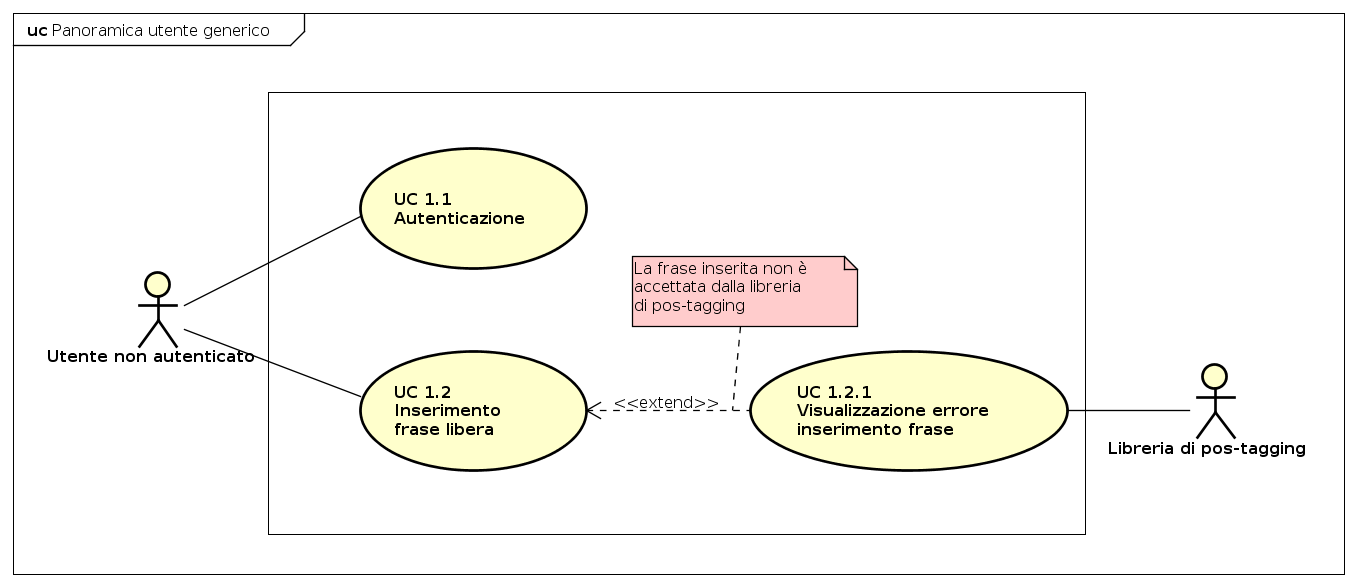
\includegraphics[width=17cm]{img/PanoramicaUtenteGenerico.png} 
\caption{Panoramica utente generico}\label{fig:1}
\end{figure}


\subsection{UC 1.1 Autenticazione}
\begin{figure}[H]
\centering
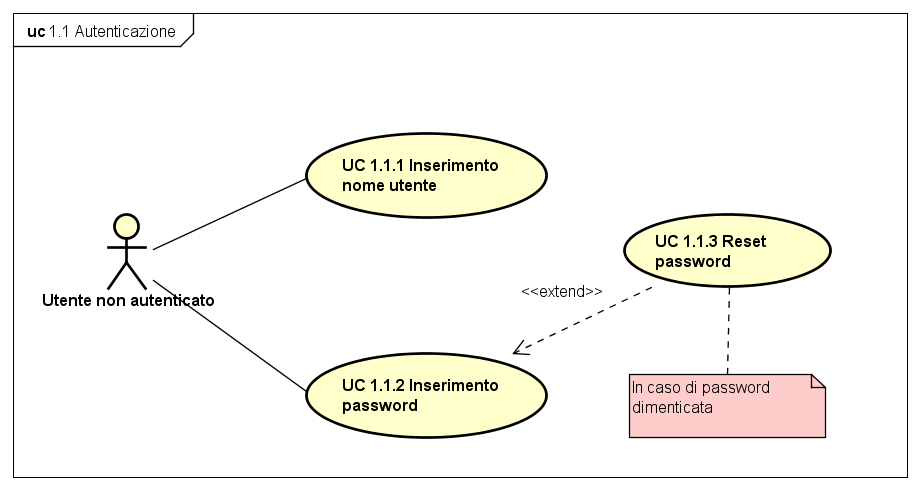
\includegraphics[width=17cm]{img/UC11.png} 
\caption{Caso d'uso 1.1}\label{fig:11}
\end{figure}
\begin{itemize}
\item[•]\textbf{Attori}: Utente non autenticato;
\item[•]\textbf{Descrizione}:  L’utente non identificato inserisce username e password e si autentica accedendo alla dashboard;
\item[•]\textbf{Precondizione}: L’utente non è autenticato;
\item[•]\textbf{Postcondizione}: L’utente viene autenticato all’interno del sistema;
\item[•]\textbf{Flusso degli eventi principale}:
\begin{enumerate}
\item UC 1.1.1 - Inserimento nome utente;
\item UC 1.1.2 - Inserimento password.
\end{enumerate}
\item[•]\textbf{Estensioni}:
\begin{enumerate}
\item Errore inserimento nome utente con relativo messaggio d’errore;
\item Errore inserimento password con relativo messaggio d’errore.
\end{enumerate}
\end{itemize}

\subsubsection{UC 1.1.1 - Inserimento nome utente}
\begin{itemize}
\item[•]\textbf{Attori}: Utente non autenticato;
\item[•]\textbf{Descrizione}: L’utente inserisce un nome utente durante la registrazione;
\item[•]\textbf{Precondizione}: L’utente non è autenticato;
\item[•]\textbf{Postcondizione}: L’utente ha inserito un nome utente;
\end{itemize}

\subsubsection{UC 1.1.2 - Inserimento password}
\begin{itemize}
\item[•]\textbf{Attori}: Utente non autenticato;
\item[•]\textbf{Descrizione}: L’utente inserisce una password durante la registrazione;
\item[•]\textbf{Precondizione}: L’utente non è autenticato;
\item[•]\textbf{Postcondizione}: L’utente ha inserito una password;
\end{itemize}

\subsection{UC 1.2 - Inserimento frase libera}
\begin{figure}[H]
\centering
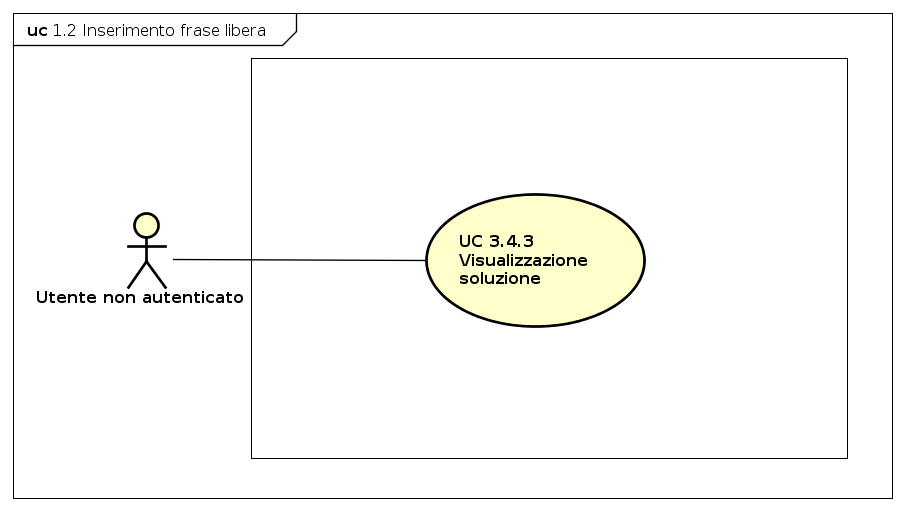
\includegraphics[width=17cm]{img/UC12.png} 
\caption{Caso d'uso 1.2}\label{fig:12}
\end{figure}
\begin{itemize}
\item[•]\textbf{Attori}: Utente non autenticato;
\item[•]\textbf{Descrizione}: L’allievo inserisce la propria frase in modo da ricevere l’analisi grammaticale di essa;
\item[•]\textbf{Precondizione}: Il sistema offre la possibilità di inserire una frase;
\item[•]\textbf{Postcondizione}: Una frase è stata correttamente inserita;
\item[•]\textbf{Flusso degli eventi principale}:
\begin{enumerate}
\item UC 3.4.3 - Visualizzazione soluzione.
\end{enumerate}
\item[•]\textbf{Estensioni}:
\begin{enumerate}
\item UC 1.2.1 - Visualizzazione errore inserimento frase.
\end{enumerate}
\end{itemize}

\subsubsection{UC 1.2.1 - Visualizzazione errore inserimento frase}
\begin{itemize}
\item[•]\textbf{Attori}: Utente non autenticato, Libreria di pos-tagging;
\item[•]\textbf{Descrizione}: La frase inserita non è accettata dalla libreria di pos-tagging. L'allievo visualizza un errore e può inserire una nuova frase;
\item[•]\textbf{Precondizione}: L’allievo ha provato ad inserire una frase;
\item[•]\textbf{Postcondizione}: L’allievo ha visualizzato il messaggio di errore e può inserire una nuova frase;
\end{itemize}
